\subsection{Limitations of Manual Software Testing}

A crucial aspect of software development is ensuring that the written code behaves as intended.  Today, this is particularly important, as software is playing an increasingly dominant role in our lives, from keeping our private data in the cloud to powering our ubiquitous smartphones.

Ideally, software would be written correctly by construction.  This was the way software engineering was envisioned in the early days of computer science~\cite{dijkstra1976discipline}; the code would be written together with the mathematical proof of its correctness.

However, the decades of software development experience that followed have painted a different picture.  As it turns out, the software complexity---up to hundreds of millions of lines of code---and rapid pace of feature development have precluded a formal, rigorous approach.
%
With the exception of a few safety-critical segments, such as avionics~\cite{Astree}, automotive~\cite{automotive}, or medical equipment, most of the software industry today relies on \emph{testing} for its quality assurance~\cite{softwareMetrics}.

Testing a program consists of exercising multiple different paths through it and checking whether ``they do the right thing.''
%
In other words, testing is a way to produce partial evidence of correctness, and thus increase confidence in the tested software.
%
Yet, test suites provide inadequate coverage of all the inputs a program could handle.
%% Yet, due to the typically poor coverage one can get today, testing often turns into a mere hunt for bugs.
%
For instance, the test suite of the Chromium browser contains about one hundred thousand tests~\cite{chrome-tests}.  This suite is thoroughly comprehensive by industry standards, yet it represents only a small fraction of all possible inputs the browser may receive.

%% In practice, most software test harnesses consist of manually written tests that are run periodically; regression test suites provide an automated way of checking whether new bugs have entered the code~\cite{codeComplete}.
%
Test suites also tend to be tedious to write and maintain.  Statistics show that, on average, developers spend as much as half of their time doing testing~\cite{codeComplete}, and companies allocate up to a quarter of their IT budget for software testing~\cite{capgemini-world-quality}.

The net result is that, despite the effort and resources invested in manual testing, bugs escape quality assurance and make it into production~\cite{redHatSecurityX}.
%
The industry average for bug density is a staggering 15 errors per 1000 lines of shipped code, while the most thorough quality assurance processes reach 0.1 errors per 1000 lines of code~\cite{codeComplete}.

Today, this problem is amplified by having an increasing number of businesses online and hence vulnerable to remote attacks that exploit software vulnerabilities.  For instance, in 2014, there were 19 vulnerabilities with CVEs reported on average \emph{per day}~\cite{nvd}.
%
These vulnerabilities are exploited to cause major disruptions~\cite{sony-hack} or leaks of sensitive data~\cite{sony-hack,psp-hack}.  On average, a data breach cost \$3.8 million in 2015~\cite{breach2015}, and the most prominent cases cost over \$100 million~\cite{target-hack}.

Alas, with a few exceptions---e.g., seL4~\cite{seL4}, a recent effort of formally verifying an operating system kernel---switching to a formal development model is not feasible for most of the software written today.
%
Despite recent advancements in formal techniques and tools, which have brought down the cost of building formally-proven software, it still takes on the order of person-years to develop a few thousand lines of verified code~\cite{seL4}.
%
This rate is currently unsustainable for most commodity software.
%
Therefore, the second best option today is to automate the software testing process itself.


\subsection{Automated Testing: Black-box vs. White-box}

The simplest (and most popular) form of automated testing consists of randomly generating program inputs and observing whether the program crashes~\cite{fuzz,quickcheck,afl,autodafe,skipfish}.
%
The inputs are typically obtained by fuzzing~\cite{fuzz}, i.e., randomly mutating a known valid input, such as an image file or a productivity suite document.  This form of testing is called ``blackbox'', because the input generation does not take into account the structure of the program under test~\cite{blackbox-testing}.
%
Despite their conceptual simplicity, fuzzers are effective at discovering  bugs~\cite{afl,autodafe,skipfish} (albeit shallow) and are currently the state of the practice in automated testing.

\begin{figure}
  \centering
  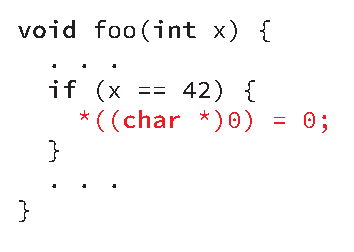
\includegraphics[width=2.0in]{introduction/figures/fuzzing-example}
  \caption{Example program for which random fuzzing is unlikely to uncover the memory error bug (the red line).}
  \label{fig:intro:fuzzing}
\end{figure}

However, plain random fuzzers are ineffective at discovering corner-case bugs---bugs that manifest only under particular inputs in the program.
%
Consider the simple example in Figure~\ref{fig:intro:fuzzing}, where the program checks the input for the particular value 42 before performing a null-pointer access.  A random fuzzer has \emph{less than a one in a billion} chance of hitting the bug with each input generated.
%
The vast majority of the generated inputs are therefore redundant.

A better approach is ``greybox'' testing, i.e., to generate tests that follow a certain structure, as defined by a specification, such as protocol format~\cite{sulley}, grammar~\cite{quickcheck}, or input precondition~\cite{boyapati:korat}.
%
However, this method would still likely miss bugs whose triggering inputs are not exposed in the input specification.

The most precise approach is to take the program structure itself into account when generating inputs.
%
This form of testing is called ``whitebox''; its goal is to generate inputs that take the program along previously unexplored execution paths.
%
Symbolic execution is the most successful automated whitebox testing technique to be applied to commodity software, in terms of size of software and bugs found~\cite{sage2012,all-symbex,decades-symbex,practice-symbex}.

\subsection{Systematic Path Exploration Using Symbolic Execution}
\label{sec:intro:symbex}

\begin{figure}
  \centering
  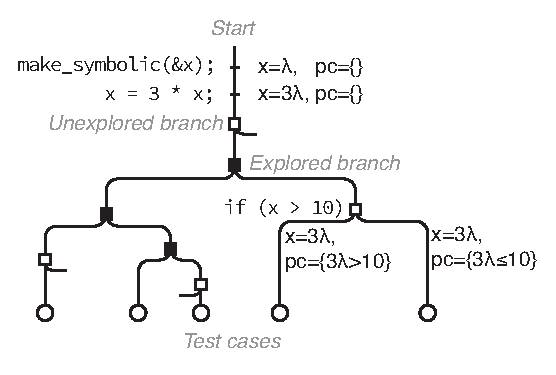
\includegraphics[width=3.5in]{introduction/figures/symbex-tree}
  \caption{Symbolic execution tree for a simple example.  Program states maintain symbolic values for variable \codebit{x} and carry a path condition (pc).}
  \label{fig:intro:symbex-tree}
\end{figure}

Symbolic execution works by executing a program with \emph{symbolic} instead of concrete input values, to cover the entire input space and thus all possible program execution paths (Figure~\ref{fig:intro:symbex-tree}).  For instance, a function \codebit{foo(int x)} is executed with a symbolic variable $\lambda$ assigned to \codebit{x}.
%
Statements using \codebit{x} manipulate it symbolically: \codebit{x := x * 3} updates the value of \codebit{x} to $3 \cdot \lambda$.  During execution, the assignment of variables to expressions is kept in a \emph{symbolic store} of the program execution state.

Whenever the symbolic execution engine encounters a conditional branch, the execution state forks into two states, whose executions proceed independently.  For each state, this process repeats for subsequent branches, turning an otherwise linear execution into a \emph{symbolic execution tree}.

Each program state keeps the conjunction of the branch conditions taken as a \emph{path condition}.
%
The path condition is a formula over the symbolic program inputs, whose solutions are concrete input assignments (e.g., $\lambda = 42$) that take the program along the same execution path.
%
The satisfiability of the formula is decided by a constraint solver, which is typically an external off-the-shelf tool~\cite{stp,Z3,cvc}.
%
The symbolic execution engine queries the solver whenever it needs to decide the feasibility of each branch condition, or when it generates a \emph{test case} at the end of an execution path.

Symbolic execution is \emph{complete}, as it systematically enumerates all program paths.
%
It is also \emph{sound}, because each execution path corresponds to a real execution, replayable using a test case.
%
The two properties make symbolic execution highly effective at automatically generating high-coverage test suites~\cite{klee}, finding bugs~\cite{sage2012,mayhem}, and even debugging~\cite{esd,oasis,portend,king:symbolic:2}.

% The satisfiability problem is NP-complete, which means there is no efficient (polynomial) algorithm available.  In practice, modern solvers can handle most formulas efficiently by using heuristics.  However, symbolic execution time is still dominated by constraint solving, as formulas can quickly become complex for non-trivial software.

%% The number of paths in the symbolic execution tree is roughly exponential in the number of program branches, with loops making the problem even worse.  As any non-trivial software can have at least thousands of branches, the size of the tree quickly becomes too large to be exhaustively covered in a reasonable amount of time.  This is called the ``path explosion'' problem.

Alas, symbolic execution is challenging to apply to non-trivial software.
%
The number of paths in the symbolic execution tree is roughly exponential in the number of program branches, with loops further amplifying the problem.  Even for moderately sized programs with hundreds of branches, the size of the execution tree becomes too large to be completely covered in a reasonable amount of time.
%
This is commonly known as the ``path explosion'' problem~\cite{burnim2008heuristics,klee,godefroid:compdyntest,rwset,state-merging}.
%
In practice, given a limited time budget, most symbolic execution engines resort to prioritizing paths guided by a pluggable engine component called a \emph{search strategy}~\cite{burnim2008heuristics,hct,dart,klee,godefroid:fuzz}.


\subsection{The Environment Problem in Symbolic Execution}

In practice, large systems can be efficiently executed symbolically by exploiting their modularity and thus symbolically execute the different parts of the system separately.
%
However, a component typically depends on its environment to perform its task.
%
This aspect is commonly encountered in the real world, where programs interact with the operating system, web applications use libraries, and so on.  Thus, we refer to this software as \emph{real-world}:

\begin{framed}
  In this thesis, we define \textbf{real-world software} as programs whose logic \emph{depends} on external functionality, such as libraries or the operating system.
  %
  We call this external functionality the \emph{environment} of the program, with which the program interacts through an environment \emph{interface}.
\end{framed}

To execute real-world software, a symbolic execution engine needs to provide the interface of its environment.
%
To reap the benefits of modularity, the engine should provide an interface that is more efficient than simply running the entire system symbolically.
%
At the same time, the engine should maintain accuracy and completeness, in order to avoid missing program paths or introducing false positives.  This conundrum is known as \emph{the environment problem}~\cite{klee}:

\begin{framed}
  The \textbf{environment problem} in symbolic execution is the trade-off between achieving \emph{efficiency} and maintaining soundness and completeness in the target program when providing its environment interface.
\end{framed}

While it also affects other program analysis techniques, such as static analysis~\cite{slam-project} and software model checking~\cite{visser-jpf}, the environment problem is particularly challenging for symbolic execution~\cite{klee,unit-system}, because of the environment complexity combined with the accuracy and completeness requirements.

First, the size of the environment---code and state---may be much larger than the size of the program itself.
%
For instance, consider a 50 lines of code system utility that prints on the terminal the contents of a file.  To perform this task, the program calls the operating system for accessing files and printing on the screen, implemented in tens of thousands of lines of kernel and library code.

Second, the environment is often stateful and its state is closely coupled with the program state.
%
In our previous example, the kernel keeps the open file and the terminal in a file table, whereas the program keeps file descriptors that index into the file table.

More sophisticated systems maintain even stronger relationships with their environments.
%
For instance, the functionality of a web server depends on the connection state and semantics of network sockets, on the memory management logic, the concurrency model, etc. as provided by the operating system and the C library.

%% The existing path explosion mitigation techniques do not suffice for efficient symbolic execution of real-world software.
%% %
%% On the one hand, executing a real-world program soundly and completely involves running the program together with its environment.
%% %
%% On the other hand, the symbolic execution engine would end up mostly executing the implementation details of the environment and make little progress inside the target program.

One simple approach for dealing with the environment problem is to let the calls into the environment go through concretely.
%
For instance, the symbolic parameters of a system call could be forcefully assigned concrete values satisfying the path condition, before executing the system call.  However, this approach risks introducing inconsistencies in the execution and miss feasible paths in the target program itself.
%
For example, if opening a file with a symbolic name would succeed or fail depending on whether the file exists or not, concretizing to an existing file name would cause the symbolic execution to miss the error handling path in the program.
%
For this example, a possible approach to simplifying the environment, while maintaining program coverage, is to employ fault injection at the environment interface: the symbolic execution engine forces the system call to both succeed and return a failure code, to exercise both successful and failing paths in the program.

\newcommand{\cnineccolor}{\cellcolor{GreenYellow}}
\newcommand{\chefccolor}{\cellcolor{SkyBlue}}

\begin{table}
  \centering
  \small
  \begin{tabular}{r p{6cm} p{6cm}}
    
    \textbf{Abstraction} & Shallow & Deep \\
    \hline
    \bigskip Examples      & Library of arbitrary-precision numbers exposed as buffers of digits to C programs.     & Native arbitrary-precision datatypes in dynamic languages (e.g., Python). \\
    
    \textbf{Encapsulation} & Weak & Strong \\
    \hline
    \bigskip Examples      & Linux file system implemented as a kernel module.   & Linux file system implemented using the FUSE user-space interface. \\
    
    \textbf{Stability}   & Stable    & Frequently-changing \\
    \hline
        Examples          & A web application that uses a standard web interface, such as CGI.    & A web application that uses the fast-changing native API of its web server (e.g., Apache). \\
  \end{tabular}
  \caption{Examples of environment interfaces, classified along main axes---abstraction and encapsulation---and stability in time.
%% Color overlays indicate design space coverage by \colorbox{GreenYellow}{\cnine} and \colorbox{SkyBlue}{\chef}.
}
  \label{tab:intro:env}
\end{table}

In general, systematically addressing the environment problem is challenging, as its manifestations depend on the nature of the environment interface and its implementation.

To broadly structure the problem space, we classify in Table~\ref{tab:intro:env} the instances of the environment problem along three main axes of the environment interface: abstraction, encapsulation, and interface stability in time.
%
Abstraction and encapsulation are two essential principles in system design.  For environments, abstraction refers to hiding the environment state behind simpler entities.
%
Encapsulation refers to restricting access to the environment state through narrow, well-defined interfaces.
%
Finally, interface stability refers to the frequency of changes in the interface specification.  For instance, well-documented and standardized interfaces tend to change less often.

For each combination of the three axes, a symbolic execution engine needs to approach the environment problem in different ways.
%
To give a sense of the environment diversity, Table~\ref{tab:intro:env} provides concrete examples for each level of abstraction, encapsulation, and stability occurring in real-world software.


%%% Local Variables: 
%%% mode: latex
%%% eval: (visual-line-mode)
%%% fill-column: 1000000
%%% TeX-master: "main"
%%% End: 
